\section{RESULTADOS E DISCUSSÃO}
  Realizamos a coleta de dados no dia 26 de junho de 2025, entre 08:05 e 08:14 (horário local). Em apenas 9 minutos de atividade, registramos 6 tentativas de login voluntárias por parte dos estudantes. Posteriormente, exportamos esses dados para CSV e realizamos o processamento para gerar as estatísticas e visualizações que apresentamos a seguir.

  \subsection{Padrões Observados}
    Nesta etapa, buscamos identificar comportamentos e tendências nos dados coletados. Observamos atentamente o perfil dos dispositivos, os navegadores utilizados e a distribuição temporal dos acessos.

    \subsection{Perfil de Dispositivos}
    Ao analisarmos o perfil dos dispositivos (Figura~\ref{fig:devices}), notamos uma distribuição curiosamente equilibrada. Metade dos acessos proveio de estações de trabalho (Desktops Windows e macOS), enquanto a outra metade originou-se de dispositivos móveis (Android e iOS). Esse equilíbrio nos chamou a atenção, pois sugere que a vulnerabilidade não está restrita a um tipo específico de acesso: tanto usuários em estações fixas quanto aqueles em trânsito interagiram com nosso portal falso.

    \begin{figure}[H]
    \centering
        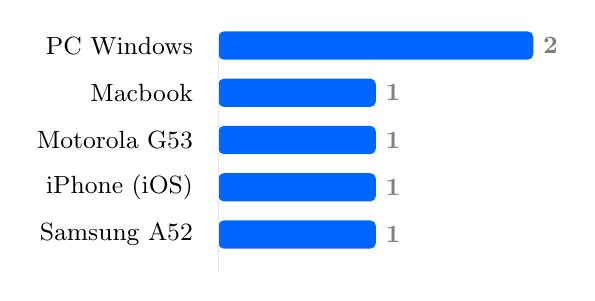
\begin{tikzpicture}[yscale=0.6]
        % Dados: valor/{Nome do Dispositivo}
        \foreach \val/\name [count=\i] in {2/{PC Windows}, 1/{Macbook}, 1/{Motorola G53}, 1/{iPhone (iOS)}, 1/{Samsung A52}} {
            \fill[blue!60!cyan, rounded corners=2pt] (0,-\i) rectangle (\val*2, -\i+0.6);
            \node[left, font=\small] at (-0.2, -\i+0.3) {\name};
            \node[right, font=\small\bfseries, gray] at (\val*2, -\i+0.3) {\val};
        }
        % Linha lateral discreta
        \draw[gray!20] (0,-0.5) -- (0,-5.5);
    \end{tikzpicture}
    \caption{Distribuição de dispositivos.}
     \label{fig:devices}
     \par\vspace{0.2cm}
     \small \textbf{Fonte:} Os autores.
\end{figure}



    Identificamos que 50\% dos acessos partiram de desktops e 50\% de dispositivos móveis, o que reforça nossa percepção de que as ações de conscientização precisam ser abrangentes e multiplataforma.

\subsubsection{Perfil de Navegadores}
\begin{figure}[H]
    \centering
    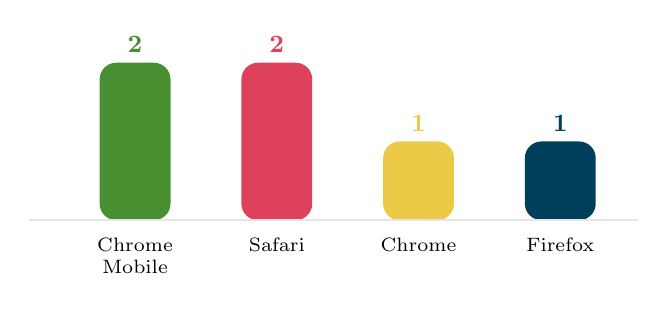
\begin{tikzpicture}[xscale=1.8]
        % Paleta de cores modernas
        \definecolor{color1}{HTML}{488f31}
        \definecolor{color2}{HTML}{de425b}
        \definecolor{color3}{HTML}{edc948}
        \definecolor{color4}{HTML}{003f5c}
    
        % Dados: {valor/rótulo/cor}
        \foreach \val/\name/\c [count=\i] in {2/{Chrome\\Mobile}/color1, 2/{Safari}/color2, 1/{Chrome}/color3, 1/{Firefox}/color4} {
            
            % Barra estilo pílula (Ponta arredondada)
            \fill[\c, rounded corners=6pt] (\i,0) rectangle (\i+0.5, \val);
            
            % Valor acima da barra
            \node[above, font=\small\bfseries, \c] at (\i+0.25, \val) {\val};
            
            % Rótulo abaixo (com quebra de linha se necessário)
            \node[below, font=\scriptsize, align=center] at (\i+0.25, -0.1) {\name};
        }
        
        % Linha de base decorativa
        \draw[gray!20, thick] (0.5,0) -- (4.8,0);
    \end{tikzpicture}
    \caption{Distribuição dos navegadores.}
    \par\vspace{0.2cm}
    \small \textbf{Fonte:} Os autores.
\end{figure}

    Verificamos que a família Chrome (somando versões mobile e desktop) foi responsável por metade dos acessos. Safari e Firefox completaram a lista, evidenciando a hegemonia das engines Chromium e WebKit entre os participantes.

\subsubsection{Distribuição por Sistema Operacional}
\begin{figure}[H]
  \centering
  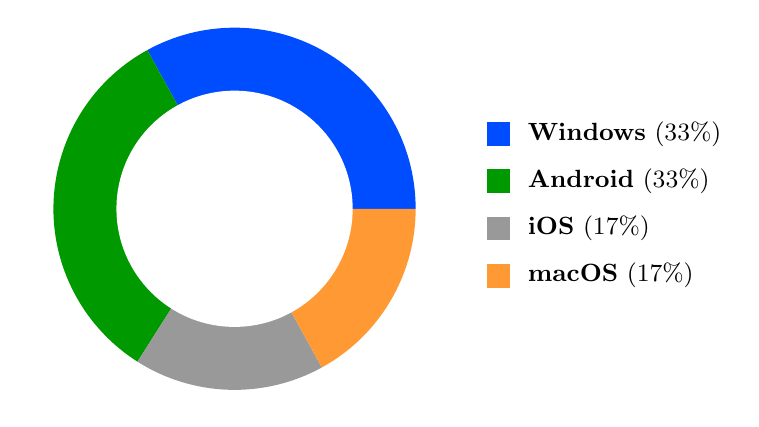
\begin{tikzpicture}
    % Fatias (Donut) usando cores padrão do TikZ/LaTeX
    % Windows - 33% (0 a 118.8 graus)
    \fill[blue!70!cyan] (0,0) -- (0:2.3) arc (0:118.8:2.3) -- cycle;
    % Android - 33% (118.8 a 237.6 graus)
    \fill[green!60!black] (0,0) -- (118.8:2.3) arc (118.8:237.6:2.3) -- cycle;
    % iOS - 17% (237.6 a 298.8 graus)
    \fill[black!40] (0,0) -- (237.6:2.3) arc (237.6:298.8:2.3) -- cycle;
    % macOS - 17% (298.8 a 360 graus)
    \fill[orange!80] (0,0) -- (298.8:2.3) arc (298.8:360:2.3) -- cycle;

    % Buraco central (efeito Donut)
    \fill[white] (0,0) circle (1.5);

    % Legenda Lateral Organizada
    \begin{scope}[shift={(3.2, 0.8)}]
      \fill[blue!70!cyan] (0,0) rectangle (0.3,0.3) node[right, black] at (0.4, 0.15) {\small \textbf{Windows} (33\%)};
      \fill[green!60!black] (0,-0.6) rectangle (0.3,-0.3) node[right, black] at (0.4, -0.45) {\small \textbf{Android} (33\%)};
      \fill[black!40] (0,-1.2) rectangle (0.3,-0.9) node[right, black] at (0.4, -1.05) {\small \textbf{iOS} (17\%)};
      \fill[orange!80] (0,-1.8) rectangle (0.3,-1.5) node[right, black] at (0.4, -1.65) {\small \textbf{macOS} (17\%)};
    \end{scope}
  \end{tikzpicture}
  \caption{Proporção de sistemas operacionais.}
  \par\vspace{0.2cm}
  \small \textbf{Fonte:} Os autores.
\end{figure}

    Observamos uma liderança compartilhada entre Windows e Android, cada um com 33\% dos acessos, refletindo a popularidade dessas plataformas no ambiente acadêmico.

\subsubsection{Classificação Mobile vs Desktop}
\begin{figure}[H]
  \centering
  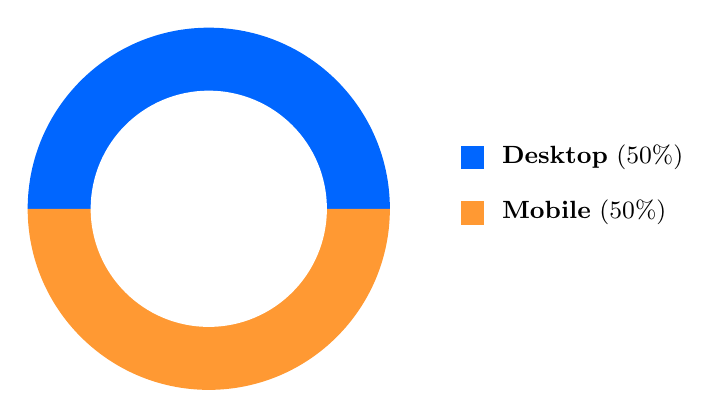
\begin{tikzpicture}
    % Fatias (Donut) - 50% cada (180 graus)
    % Desktop - Azul
    \fill[blue!60!cyan] (0,0) -- (0:2.3) arc (0:180:2.3) -- cycle;
    % Mobile - Laranja/Âmbar
    \fill[orange!80] (0,0) -- (180:2.3) arc (180:360:2.3) -- cycle;

    % Buraco central (efeito Donut)
    \fill[white] (0,0) circle (1.5);

    % Legenda Lateral Organizada
    \begin{scope}[shift={(3.2, 0.5)}]
      \fill[blue!60!cyan] (0,0) rectangle (0.3,0.3) 
        node[right, black] at (0.4, 0.15) {\small \textbf{Desktop} (50\%)};
      
      \fill[orange!80] (0,-0.7) rectangle (0.3,-0.4) 
        node[right, black] at (0.4, -0.55) {\small \textbf{Mobile} (50\%)};
    \end{scope}
  \end{tikzpicture}
  \caption{Acessos: mobile vs desktop.}
  \par\vspace{0.2cm}
  \small \textbf{Fonte:} Os autores.
\end{figure}

    A divisão exata entre mobile e desktop foi um achado importante para nossa equipe, confirmando que não devemos negligenciar nenhum dos dois segmentos em futuras campanhas educativas.

\subsubsection{Distribuição Temporal dos Acessos}
\begin{figure}[H]
  \centering
  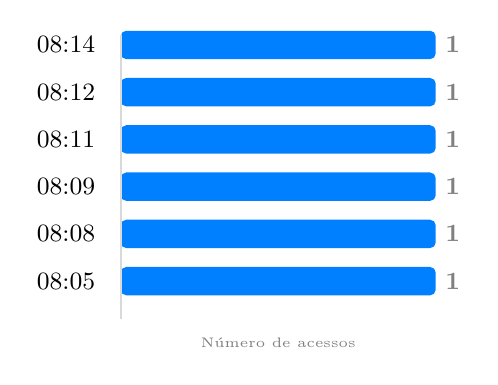
\begin{tikzpicture}[yscale=0.6]
    % Dados: valor/{Horário}
    \foreach \val/\name [count=\i] in {1/{08:14}, 1/{08:12}, 1/{08:11}, 1/{08:09}, 1/{08:08}, 1/{08:05}} {
        
        % Barras horizontais (valor * 4 para dar largura, já que todos são 1)
        \fill[blue!50!cyan, rounded corners=2pt] (0,-\i) rectangle (\val*4, -\i+0.6);
        
        % Horários à esquerda
        \node[left, font=\small] at (-0.2, -\i+0.3) {\name};
        
        % Valor numérico ao final da barra
        \node[right, font=\small\bfseries, gray] at (\val*4, -\i+0.3) {\val};
    }
    % Linha de base vertical sutil
    \draw[gray!30, thick] (0,-0.5) -- (0,-6.5);
    
    % Rótulo do eixo X (opcional, para clareza)
    \node[font=\tiny, gray] at (2, -7) {Número de acessos};
  \end{tikzpicture}
  \caption{Acessos por minuto entre 08:05 e 08:14.}
  \par\vspace{0.2cm}
  \small \textbf{Fonte:} Os autores.
\end{figure}

  Notamos que os acessos ocorreram de forma distribuída ao longo dos 9 minutos, sem picos repentinos. Isso sugere que a participação foi orgânica e voluntária, e não fruto de um efeito de “manada”.

 \subsection{Análise de Padrões}
     \begin{itemize}
       \item \textbf{Prevalência do Chrome:} A forte presença do Chrome nos faz refletir sobre a importância de verificar configurações de segurança em navegadores baseados em Chromium.
       \item \textbf{Equilíbrio de plataformas:} Concluímos que qualquer política de segurança deve tratar usuários móveis e de desktop com igual prioridade.
       \item \textbf{Espontaneidade:} A distribuição temporal dos acessos reforçou nossa confiança de que os dados coletados refletem um comportamento real dos usuários.
     \end{itemize}